\documentclass[10pt]{book}
\usepackage[paperwidth=6in, paperheight=9in,bindingoffset=5mm,%having an inner margin offset prevents text falling into the gutter
inner=20mm,
outer=20mm,
top=20mm,
bottom=21mm,
twoside,
heightrounded]{geometry}

%Basic English formatting:
	\frenchspacing %Prevents the silly double space after each sentence
	\usepackage{pifont} %Needed for \ding characters (for the crosses mainly)
	\usepackage{ebgaramond} %Standard open source font
	\setlength{\parindent}{1em}
	
%To ensure language compatibility.
	\usepackage[utf8]{inputenc}
	\usepackage[greek,latin,british]{babel}

%To change tracking and tighten up spacing:
	\usepackage{microtype}
	
%To contain Apostles' Creed and other minibox:
\usepackage{adjustbox}

%Makes sure odd pages are on the right when moving between page number types.
	\usepackage[strict]{changepage}
	\usepackage{scrextend}
	
%URL
	\usepackage[hidelinks]{hyperref}	

%Page Headers
	\usepackage{fancyhdr}
	\pagestyle{fancy}
	\fancyhf{}
	\renewcommand{\headrulewidth}{0pt} %Prevent line at top of page
	\fancyfoot[C]{\thepage}
%Prevents chapter from resetting page layout
	\fancypagestyle{plain}{
		\fancyhf{}
		\fancyfoot[C]{}
		\renewcommand{\headrulewidth}{0pt}}
		


%Try to avoid warnings:
\setlength{\headheight}{17.13pt}


%Change section format:
\setcounter{secnumdepth}{0} %Remove section numbering
	\usepackage{titlesec}
	\titleformat{\section} % Command to modify
		{\Large \normalfont \centering} % Format
  		{} % No label (removes number)
  		{0pt} % Spacing between label and title (irrelevant here since no label)
  		{}
	
	\titleformat{\subsection}
	{\normalsize\bfseries\scshape\centering}
  	{}
  	{0pt}
	{}
	
	\titleformat{\subsubsection}
	{\normalsize\centering\itshape}
  	{}
  	{0pt}
	{}

%Colour \& Images

	%Image Configuration
	\usepackage{graphicx}
	\graphicspath{{resources/images}}
	\usepackage{wrapfig}
	\usepackage{epsfig}
	
	%For Devotional Hymns
	\usepackage{pdfpages}

	%Enables text under image without caption.
	\usepackage{caption}
	\captionsetup[figure]{labelformat=empty,justification=centering}
	\usepackage{float}

	%Colour
	\usepackage[svgnames,dvipsnames]{xcolor}

	%Changes to the Table of Contents
	\addto\captionsbritish{\renewcommand{\contentsname}{Table of Contents}}
	\setcounter{tocdepth}{1} %Only chapters & sections are added to the TOC
	\usepackage{tocloft}
	\setlength{\cftbeforetoctitleskip}{-8ex}

	%For quotations in the Foreword and Editor's Preface:
	\usepackage{quoting}

	%For the signature in the Preface \& Margins
	\usepackage{ragged2e}

	%For the Chant Notation
	\usepackage[autocompile]{gregoriotex}
	
	%Special cross
	\gresetspecial{cross}{\grealtcross}
	
	%I'm not sure what this does.
	\gresetheadercapture{initial-style}{gresetinitiallines}{}

%For smaller subsections in the Hymnal Copyright page:
\newcommand{\hcopyrightsection}[1]{\par\centerline{\textbf{\small#1}}\par}

%Rubrics:
	%Colour for print:
	\definecolor{RubricRed}{cmyk}{0, 1, 1, 0.4}

	%For black words in rubrics.
	\newcommand{\blackrubric}[1]{{\color{black}#1}}
	
	%Heading Rubrics
	\newenvironment{inhead}{\par\centering\color{RubricRed}\small\smallskip\ignorespaces}
	{\par\normalsize\smallskip\ignorespacesafterend}
	
	%Normal Rubrics
	\newenvironment{rubric}{\par\smallskip\par\noindent\color{RubricRed}\small\ignorespaces\P}
		{\par\normalsize\smallskip\ignorespacesafterend}
		
	%For rubrics right after sections
	\newenvironment{secrubric}{\par\noindent\small\ignorespaces\color{RubricRed}\P}
	{\par\normalsize\smallskip\ignorespacesafterend}
	
	%Inline Rubric
	\newcommand{\inrub}[1]{{{\color{RubricRed}\small(#1)}}}
	
	%Determine Marginnote parameters
	\setlength{\marginparwidth}{15mm} % Set the width of the margin note
	\setlength{\marginparsep}{2mm} % Set the spacing between the margin note and the text
	\usepackage{marginnote}

	%Margin Rubric on Odd Pages
	
	\newcounter{alphacount} %Counter to convert number to letter
\newcommand{\margrub}[2]{\setcounter{alphacount}{#1}\textsuperscript{\alph{alphacount}}%
	\marginpar{\begin{minipage}{0.65\marginparwidth}
	\sloppy%
	\itshape%
	\scriptsize%
	\textsuperscript{\alph{alphacount}}%
	#2
	\fussy
	\end{minipage}}
  \hspace{-0.2em}}
 
  
  	%Margin Rubric on Even Pages
  \newcommand{\margrubleft}[2]{\setcounter{alphacount}{#1}\textsuperscript{\alph{alphacount}}%
	\marginpar{\RaggedLeft%
	\sloppy%
	\itshape%
	\scriptsize%
	\textsuperscript{\alph{alphacount}}%
	#2%
	\fussy}
  	\hspace{-0.2em}}
  
  	%Margin Rubric in Column Contexts (English Column)
  \newcommand{\margcolrub}[2]{\setcounter{alphacount}{#1}%
	\textsuperscript{\alph{alphacount}}%
	\Ifthispageodd{\reversemarginpar
	\marginpar{%
	\raggedright%
	\sloppy%
	\itshape%
	\scriptsize%
	    \textsuperscript{\alph{alphacount}}%
	    #2\hspace{-0.2em}%
	    \fussy}
	    }{\normalmarginpar
	    \marginpar{%
		\raggedleft%
		\sloppy%
		\itshape%
		\scriptsize%
		\textsuperscript{\alph{alphacount}}%
	    #2\hspace{-0.2em}%
	    \fussy}}}
  
  %Really just a placeholder in case it becomes relevant later in the latin side of a double column:
  \newcommand{\marglatincolrub}[2]{\setcounter{alphacount}{#1}\textsuperscript{\alph{alphacount}}\hspace{-0.2em}}
	
		%Margin Rubric without letter/number.
	  \newcommand{\margy}[1]{\marginpar{\RaggedRight%
		\sloppy%
		\itshape%
		\scriptsize%
		#1%
		\fussy}}
		
		%Margin Rubric without letter/number, on the left side (even numbered page).
	  	\newcommand{\margyleft}[1]{\marginpar{\RaggedLeft%
		\sloppy%
		\itshape%
		\scriptsize%
		#1%
		\fussy}}
  
  
		
	  
	%Kalendar \& Lectionary
	\usepackage{array}
	\usepackage{longtable} %Allows lectionary cells to go over multiple pages
	\newcolumntype{C}[1]{>{\centering\arraybackslash}p{#1}}
	\newcolumntype{L}[1]{>{\RaggedRight\arraybackslash}p{#1}}
	
		%Lectionary Evensong
		\newcommand{\evensong}[1]{Evensong}
	
	%Scriptural Citations in Mass
	\newcommand{\vr}[1]{{\footnotesize{ (#1)}}}
	
	%Disable \vr
	\newcommand{\novr}[1]{}
	
	%Invitatory
	\newcommand{\inv}[1]{{\color{RubricRed}#1.}}

%Propers:

	%Drop Caps (And specifies a specific folder for normal lettrine images):
	\usepackage{lettrine}
	\newcommand{\lett}[2]{\lettrine[image=true,realheight=true,lines=3]{dropcaps/#1.png}{{\lowercase{#2}}}}
	
	%If no second or third lines, and line amount might be doubtful, then this is used to ensure adequate spacing.
	\newcommand{\lettspace}[0]{\ifnum\prevgraf=1
		\vspace{2\baselineskip}
			\else
				\ifnum\prevgraf=2
					\vspace{1\baselineskip}
				\fi
			\fi}
	

%Replacing page references, now that the Book of Common Prayer is now published. The Missal page numbers will be added once that is published.

\newcommand{\SPMaryAdvent}{BCP 541}
\newcommand{\SPMaryChristmas}{BCP 541}
\newcommand{\SPMaryEaster}{BCP 542}
\newcommand{\SPSaints}{BCP 542}
\newcommand{\SPAgainst}{BCP 543}
\newcommand{\SPChiefBishop}{BCP 543}
\newcommand{\SPHolyGhost}{BCP 544}
\newcommand{\SPLiving}{BCP 544}
\newcommand{\Lammas}{BCP 477}
\newcommand{\AllHallows}{BCP 532}

	
	%Ensure that short paragraphs don't lead to text moving into drop cap.
	
	\newcounter{thirdlinecounter} %Counter to tell thirdline how many paragraphs precede it.
	\newcommand{\secondline}[1]{%
		\ifnum\prevgraf>2 %If there are over two lines in the previous paragraph (3), then we don't need to adjust anything, and it is put as is.
			#1\par
			\setcounter{thirdlinecounter}{3}
		\else
			\ifnum\prevgraf=2%If there are only two lines, then we only need to do an indent.
				\parindent=3.25em
				#1\par
            	\parindent=1em%Reset indent to normal
            	\setcounter{thirdlinecounter}{2}
			\else
				\ifnum\prevgraf=1%If the lett paragraph is only one line, then we need to cause the entirety of the next paragraph to be indented.
				\noindent
				\leftskip=3.25em
				#1\par
				\leftskip=0em%Reset indent to normal
				\setcounter{thirdlinecounter}{1}
					\else%In case something is not caught.
						#1
						\setcounter{thirdlinecounter}{3}
						\par
				\fi
			\fi
		\fi}
	
	%Make sure proper formatting for the third line.
	\newcommand{\thirdline}[1]{\addtocounter{thirdlinecounter}{\prevgraf}%
		\ifnum\thethirdlinecounter=2%If there are only two lines preceding (one line of the lett and one line of the secondline
    		\parindent=3.25em
    		#1\par
    		\parindent=1em
				\else
	    		#1\par
		\fi}
	
	\usepackage[super]{nth} %To add superscript to ordinal numeral.
	
	%Rank, Date, Name for Feast Days
	\newcommand{\festival}[3]{\par\subsection{#2. #3}
	
	\begin{inhead}
		#1
	\end{inhead}}
	
	
%For typesetting Memorials
\newcommand{\subbymemorial}[2]{%
\subsection{(#1. #2)}}

%To indicate and format a Festival already in the Book of Common Prayer:
\newcommand{\bcpfeast}[3]{\subsection{[#1]}%
%Feast Day:
\fancyhead[RO,LE]{\textit{#2}}%
%Feast Date:
\fancyhead[RE,LO]{#3}}



	%Headings for the Propers
	\newcommand{\feastday}[1]{\fancyhead[RO,LE]{\textit{#1}}} %Feast Name
	
	\newcommand{\feastdate}[2]{\fancyhead[RE,LO]{#1 #2}} %Feast Date
	
	%Psalm Numbers
	\newcommand{\psanum}[1]{{\small{#1}} }
	
	%For drawing boxes around unapproved text:
	\usepackage[most]{tcolorbox}
	
	%To make sure versicle and response start with indent.
	\usepackage{indentfirst}

	%To create hanging indent for Hymns.
	\usepackage{hanging}
	
	%Introit
	\newcommand{\introit}[0]{\subsubsection{Introit}}
	
	%Collect
	\newcommand{\collect}[0]{\subsubsection{Collect}}

	%Readings
	\newcommand{\readingcitation}[2]{\subsubsection{#1. \emph{#2}}}
	
	%Divine Name in Readings
	\newcommand{\divineName}[1]{\textsc{\lowercase{#1}}}
	
	%Gradual \& Alleluia
	\newcommand{\gradall}[2]{\gradual{#1}\par\alleluia{#2}}
	
	%Gradual \& Tract
	\newcommand{\gradtr}[2]{\gradual{#1}\par\tract{#2}}
	
	%Alleluia Verse
	\newcommand{\alleluia}[1]{\vspace{1ex}\par\noindent
		\emph{Alleluia.} #1}
	%Gradual
	\newcommand{\gradual}[1]{\vspace{1ex}\par\noindent
		\emph{Gradual.} #1}
		
	%Tract
	\newcommand{\tract}[1]{\vspace{1ex}\par\noindent
		\emph{Tract.} #1}
		
    %Offertory
    \newcommand{\offertory}[1]{\vspace{1ex}\par\noindent
		\emph{Offertory.} #1}
		
	%Secret
	\newcommand{\secret}[0]{\subsubsection{Secret}}

	%Communion
	\newcommand{\communion}[1]{\vspace{1ex}\par\noindent
    	\emph{Communion.} #1}
	
	%Postcommunion
	\newcommand{\postcommunion}[0]{\subsubsection{Postcommunion}}
		
	%Antiphons
	\newcommand{\antiphon}[2]{{\centering \textit{#1 Ant.} #2}}
	
	%Do I need?
	\newcommand{\properantiphon}[2]{{\centering \textit{#1 Ant.} #2}}
	
	%Invitatory Hymn Heading
	\newcommand{\invitatoryhymn}{%
		\begin{inhead}
			Invitatory Hymn
		\end{inhead}}

	%Office Hymn Heading
	\newcommand{\officehymn}{\par\vspace{0.1\baselineskip}%
		\begin{inhead}
			Office Hymn
		\end{inhead}
		\par
		\vspace{-0.1\baselineskip}}


\usepackage{paracol} %To provide balanced English-Latin dual paragraphs
\usepackage[grid]{multicol} %For non bilingual dual columns.
\setlength\columnseprule{0.4pt} %Controls the width of the line between columns

%Prevent lettrine misalignment:
\raggedbottom

%English-Latin Double Column
\newcommand{\elcol}[2]{\sloppy
	\begin{paracol}{2}
		\begin{leftcolumn}
			#1
		\end{leftcolumn}
		\begin{rightcolumn}
			\selectlanguage{latin}%
			#2
		\end{rightcolumn}
		\switchcolumn*
	\end{paracol}
\selectlanguage{british}
\fussy}

%English-Latin Non-Indented Column
\newcommand{\elcoldent}[2]{\sloppy
	\begin{paracol}{2}
		\begin{leftcolumn}
		\noindent%
			#1	
		\end{leftcolumn}
		\begin{rightcolumn}
                \selectlanguage{latin}%
			\noindent
			#2
		\end{rightcolumn}
		\switchcolumn*
	\end{paracol}
\selectlanguage{british}
\fussy}

%For difference between through the year and in eastertide:
\newcommand{\ttyie}[2]{\sloppy
	\begin{paracol}{2}
		\begin{leftcolumn}\noindent
			#1	
		\end{leftcolumn}
		\begin{rightcolumn}\noindent
			#2
		\end{rightcolumn}
		\switchcolumn*
	\end{paracol}
\selectlanguage{british}
\fussy}

%Expedites adding dual language Oremus/Let Us Pray
\newcommand{\oremus}[0]{\par
	\begin{paracol}{2}
		\begin{leftcolumn}
			\selectlanguage{british}\noindent%
			\centerline{\textit{Let us pray.}}
		\end{leftcolumn}
		\begin{rightcolumn}
			\selectlanguage{latin}\noindent%
			\centerline{\textit{Orémus.}}
		\end{rightcolumn}
		\switchcolumn*
	\end{paracol}
\selectlanguage{british}}

%Does the same as above, but for single language collects:
\newcommand{\letuspray}[0]{\par\noindent
	\centerline{\textit{Let us pray.}}
	\par}

\newcommand{\oremuslatin}[0]{\par\noindent
	\centerline{\textit{Orémus.}}
	\par}
	
	
	
\begin{document}
\begin{titlepage}
		\begin{center}
			{\Large{The}}
			\par
			\vspace{.4cm}
			{\Huge{\scshape Prayer Book}}
			\par
			\vspace{.4cm}
			{\Huge{\scshape Hymnal}}
			\par
			\vspace{.4cm}
			{\large{\textit{A Supplement of Hymns \& Propers for the Book of Common Prayer}}}
			\end{center}
			
			\vfill
			
			\begin{figure}[H]
				\centering
				
\includegraphics[scale=.17]{logo.eps}
				\caption{\scshape Apologia Anglicana\\Boston, Massachusetts\\
				A. D. MMXXV}
			\end{figure}
		
	\end{titlepage}
\cleardoublepage
\pagenumbering{gobble}
%~\clearpage
\tableofcontents
\addtocontents{toc}{\vspace*{-3ex}}%
\clearpage
%This is to ensure two odd-numbered pages are not right next to each other:
%\clearpage
%\checkoddpage
%\ifoddpage \else
%\fi
%Roman numeral page numbers for the front material.
\include{pages/Copyright.tex}
%\phantomsection
\addcontentsline{toc}{chapter}{Foreword}
\fancyhead[C]{{\LARGE Foreword}}
\noindent
Foreword goes here.
\phantomsection
\addcontentsline{toc}{chapter}{Editor's Preface}
\fancyhead[C]{{\LARGE Editor's Preface}}
\noindent
\begin{quoting}
	O God, my heart is ready, my heart is ready : I will sing and give praise with the best member that I have. Awake, thou lute and harp : I myself will awake right early. ---Psalm 108:1-2
\end{quoting}
\par\noindent
\lett{W}{e} are blessed to finally be able to publish the \emph{Prayer Book Hymnal}. Together with the 2025 Proposed Book of Common Prayer (or the Office book), it completes everything necessary for a full recitation of the Daily Office within the English Orthodox tradition. It provides not only the Office propers for the Seasons and Festivals---taken almost always from the Benedictine tradition---but also the Ordinary and even devotional hymns, which are especially helpful in a parish context.\\

The devotional hymns hold a special place in our hearts, for it is truly an amazing display of local piety. Our goal was to provide a selection of the best of the hymnal tradition. American Anglican hymns were given pride of place, without excluding the beautiful and well-known hymns of other traditions. We trust that it will enrich not only individual Christians but also Congregations, especially smaller ones with limited choirs.\\

In addition to the Daily Office, it was our concern that also the Holy Sacrifice of the Mass could be celebrated with the BCP when a Minor Festival needs to be celebrated or commemorated. For everything a parish may need to celebrate, Holy Week excluded for practical reasons, the BCP and the \emph{Prayer Book Hymnal} provide everything necessary.\\

As the Prayer Book Tradition matured, two kinds of `two-book' solutions developed. On the one hand, many followed the Roman tradition of dividing the Daily Office and the Holy Mass into separate books---the Missal and the Breviary (along with a Hymnal in parish contexts). On the other hand, however, due to the centrality of the Book of Common Prayer, a second `two-book' solution developed, retaining the BCP as the core and then providing supplements. It is within this tradition that the \emph{Prayer Book Hymnal} has been formed and exists.\\

While time will tell which arrangement of liturgical books will be favoured and become dominant within the English Orthodox tradition, we are confident this Book holds an important place and unique benefit for all those committed to the daily recitation of the Office and the reverent offering of the Holy Sacrifice of the Mass.\\

We hope this \emph{Prayer Book Hymnal} assists you in your prayers. Please pray for us as we pray for you and the salvation of all men.\\

\rightline{\emph{Pax Christi,}}

\rightline{Mr. Augustine Watson, MSt}

\rightline{Chief Editor, Apologia Anglicana}


%\include{pages/Dedication.tex}

%\include{pages/FrequentPrayers.tex}

%Office Hymns
\cleardoublepage
\fancyhead[RE,LO]{}\fancyhead[RO,LE]{}
\fancyhead[C]{}\thispagestyle{empty}
\mainmatter
\phantomsection
\addcontentsline{toc}{chapter}{Daily Hymns}

\begin{figure}[H]
    \centering
    
\includegraphics[width=98mm, height=140mm]{VirginMonks.eps}
    \caption{\textsc{\Huge{Daily Hymns}}}
\end{figure}
\include{pages/Propers/FerialHymns.tex}
%Liturgical Hymns
\cleardoublepage
\include{pages/Daily_Office/LiturgicalHymnsFront.tex}
\fancyhead[C]{\LARGE Liturgical Hymns}

\section{Ordinary of the Office}
\fancyhead[RO,LE]{\textit{Office Ordinary}}
	
	\subsection{Introduction}\fancyhead[RE,LO]{Introduction}
	
	\subsubsection{Simple}
	
	\noindent
	\gregorioscore{resources/gabc/MassParts/Ordinary/Simple/OpenThou.gabc}
	
	\noindent
	\gregorioscore{resources/gabc/MassParts/Ordinary/Simple/AndOur.gabc}
	
	\vspace{3ex}
	
	\noindent
	\gregorioscore{resources/gabc/MassParts/Ordinary/Simple/MakeSpeed.gabc}
	
	\noindent
	\gregorioscore{resources/gabc/MassParts/Ordinary/Simple/MakeHaste.gabc}
		
	\vspace{3ex}
	
	\noindent
	\gregorioscore{resources/gabc/MassParts/Ordinary/Simple/GloryBe.gabc}
	
	\noindent
	\gregorioscore{resources/gabc/MassParts/Ordinary/Simple/AsItWas.gabc}
		
	\vspace{5ex}
	
	\noindent
\begin{minipage}[t]{0.48\textwidth}
\noindent
	\gregorioscore{resources/gabc/MassParts/Ordinary/Simple/PraiseYe.gabc}
\end{minipage}
\hfill
\begin{minipage}[t]{0.48\textwidth}
\noindent
	\gregorioscore{resources/gabc/MassParts/Ordinary/Simple/Praised.gabc}
\end{minipage}
	
	\subsubsection{Solemn}
	
	\noindent
	\gregorioscore{resources/gabc/MassParts/Ordinary/Solemn/OpenThou.gabc}
	
	\noindent
	\gregorioscore{resources/gabc/MassParts/Ordinary/Solemn/AndOur.gabc}
	
	\vspace{3ex}
	
	\noindent
	\gregorioscore{resources/gabc/MassParts/Ordinary/Solemn/MakeSpeed.gabc}
	
	\noindent
	\gregorioscore{resources/gabc/MassParts/Ordinary/Solemn/MakeHaste.gabc}
	
	\vspace{3ex}
	
	\noindent
	\gregorioscore{resources/gabc/MassParts/Ordinary/Solemn/GloryBe.gabc}
	
	\noindent
	\gregorioscore{resources/gabc/MassParts/Ordinary/Solemn/AsItWas.gabc}
		
	\vspace{5ex}
	
	\noindent
\begin{minipage}[t]{0.48\textwidth}
\noindent
	\gregorioscore{resources/gabc/MassParts/Ordinary/Solemn/PraiseYe.gabc}
\end{minipage}
\hfill
\begin{minipage}[t]{0.48\textwidth}
\noindent
	\gregorioscore{resources/gabc/MassParts/Ordinary/Solemn/Praised.gabc}
\end{minipage}

%MANUAL ADJUSTMENT:
\clearpage
\subsection{Apostles' Creed}\fancyhead[RE,LO]{Apostles' Creed}
\par\noindent
\adjustbox{valign=t}{\noindent
\begin{minipage}[t]{0.7\textwidth}\noindent
\noindent
	\gregorioscore{resources/gabc/MassParts/Ordinary/ApostlesCreed.gabc}
\end{minipage}
}
\hfill
\adjustbox{valign=t}{
\begin{minipage}[t]{0.25\textwidth}
Maker of heaven and earth: And in Jesus Christ his only Son our Lord: Who
\end{minipage}
}

\vspace{0.5\baselineskip}
\par\noindent
	 was conceived by the Holy Ghost, Born of the Virgin Mary: Suffered under Pontius Pilate, Was crucified, dead, and buried: He descended into hell; The third day he rose again from the dead: He ascended into heaven, And sitteth on the right hand of God the Father Almighty: From thence he shall come to judge the quick and the dead.\par
    I believe in the Holy Ghost: The holy Catholic Church; The Communion of Saints: The Forgiveness of sins: The Resurrection of the body: {\ding{64}} And the Life
    \par\noindent
    \adjustbox{valign=t}{\par\noindent
\begin{minipage}[t]{0.15\textwidth}\par\noindent
everlasting.
\end{minipage}
}
\hfill
\adjustbox{valign=t}{
\begin{minipage}[t]{0.825\textwidth}
\noindent
	\gregorioscore{resources/gabc/MassParts/Ordinary/Amen.gabc}
\end{minipage}
}

    
\subsection{Salutation}\fancyhead[RE,LO]{Salutation}

	\noindent
	\gregorioscore{resources/gabc/MassParts/Ordinary/LordBeWithYou.gabc}
	
	\begin{inhead}
		or,
	\end{inhead}
	
	\noindent
	\gregorioscore{resources/gabc/MassParts/Ordinary/OLordHear.gabc}
	
\subsection{Kyrie}\fancyhead[RE,LO]{Kyrie}

	\noindent
\begin{minipage}[t]{0.48\textwidth}
\noindent
	\gregorioscore{resources/gabc/MassParts/Ordinary/LordHaveMercy.gabc}

℟. Christ, have mercy upon us.

℣. Lord, have mercy upon us.

\end{minipage}
\hfill
\begin{minipage}[t]{0.48\textwidth}
\noindent
	\gregorioscore{resources/gabc/MassParts/Ordinary/Kyrie.gabc}

℟. Christe, eléison.

℣. Kýrie, eléison.

\end{minipage}

%MANUAL ADJUSTMENT:
\clearpage
\subsection{Lord's Prayer}\fancyhead[RE,LO]{Lord's Prayer}

\noindent
	\gregorioscore{resources/gabc/MassParts/Ordinary/LordsPrayer.gabc}

\subsection{Preces}\fancyhead[RE,LO]{Preces}

\noindent
	\gregorioscore{resources/gabc/MassParts/Ordinary/Preces.gabc}

\subsection{Mattins Collects}\fancyhead[RE,LO]{Collects}

\subsubsection{A Collect for Peace}

\noindent
	\gregorioscore{resources/gabc/MassParts/Ordinary/CollectPeace.gabc}

\subsubsection{A Collect for Grace}

\noindent
	\gregorioscore{resources/gabc/MassParts/Ordinary/CollectGrace.gabc}

\subsection{Evensong Collects}

\subsubsection{A Collect for Peace}

\noindent
	\gregorioscore{resources/gabc/MassParts/Ordinary/CollectPeaceEvensong.gabc}

\subsubsection{A Collect for Aid against Perils}

\noindent
	\gregorioscore{resources/gabc/MassParts/Ordinary/CollectAid.gabc}


\subsection{Conclusion}\fancyhead[RE,LO]{Conclusion}

\noindent
	\gregorioscore{resources/gabc/MassParts/Ordinary/ClosingLordBeWithYou.gabc}

\begin{inhead}
	or,
\end{inhead}

\noindent
	\gregorioscore{resources/gabc/MassParts/Ordinary/ClosingOLordHear.gabc}

%MANUAL ADJUSTMENT:
\clearpage
    \par\noindent
	\centerline{\rule{0.25\textwidth}{0.4pt}}
	\par\noindent
\begin{rubric}
	On Ferial Days,
\end{rubric}

\noindent
	\gregorioscore{resources/gabc/MassParts/Ordinary/LetUsBlessFerial.gabc}

\begin{rubric}
	On Feast Days,
\end{rubric}

\noindent
	\gregorioscore{resources/gabc/MassParts/Ordinary/LetUsBlessFestal.gabc}


\begin{rubric}
	During Eastertide,
\end{rubric}

\noindent
	\gregorioscore{resources/gabc/MassParts/Ordinary/LetUsBlessEaster.gabc}
    \par\noindent
	\centerline{\rule{0.25\textwidth}{0.4pt}}
	\par\noindent
\begin{rubric}
	In a low voice,
\end{rubric}

\noindent
	\gregorioscore{resources/gabc/MassParts/Ordinary/FideliumAnimae.gabc}
	
	\clearpage
	\section{Office Service}\fancyhead[RO,LE]{\textit{Office Service}}
	
	\subsection{Our Worship, Praise, and Thanksgiving\\unto the Glory of God Alone}
	
		\begin{inhead}
			Mattins
		\end{inhead}
		
		\subsubsection{Venite, exultemus Domino}\fancyhead[RE,LO]{Venite}
		
			\noindent
	\gregorioscore{resources/gabc/Extra/Venite.gabc}
			
			\psanum{2}Let us come before his presence with • thanksgiving : and shew ourselves • glad in him with psalms.
			
			\psanum{3}For the Lord is a • great God : and a great • King above all gods.
			
			\psanum{4}In his hand are all the corners • of the earth : and the strength of the hills is • his also.
			
			\psanum{5}The sea is his, and • he made it : and his hands prepared • the dry land.
		
			\psanum{6}O come, let us worship and • fall down : and kneel before the • Lord our Maker.
			
			\psanum{7}For he is the • Lord our God : and we are the people of his pasture, and the • sheep of his hand.
			
			\psanum{8}To-day if ye will hear his voice, harden • not your hearts : as in the provocation, and as in the day of temptation • in the wilderness.
			
			\psanum{9}When your fathers • tempted me : proved me, • and saw my works.
			
			\psanum{10}Forty years long was I grieved with this generation, • and said : It is a people that do err in their hearts, for they • have not known my ways;
			
			\psanum{11}Unto whom I sware • in my wrath : that they should not enter • into my rest.
			
			℣. Glory be to the Father, and • to the Son * and • to the Holy Ghost.
			
			℟. As it was in the beginning, is now, and ever • shall be * world without • end. Amen.
			
	
		\clearpage\subsubsection{Pascha Nostrum}\fancyhead[RE,LO]{Pascha Nostrum}
		
			\noindent
	\gregorioscore{resources/gabc/Extra/PaschaNostrum.gabc}
	
			Not with old leaven, neither with the leaven of malice and • wickedness * but with the unleavened bread of sin • cerity and truth.
	
			Christ being raised from the dead dieth • no more * death hath no more do • minion over him.
    
    		For in that he died, he died unto • sin once * but in that he liveth, he • liveth unto God.
    
    		Likewise reckon ye also yourselves to be dead indeed • unto sin * but alive unto God through • Jesus Christ our Lord.
    
    		Christ is risen • from the dead * and become the first • fruits of them that slept.

    		For since by • man came death * by man came also the resur • rection of the dead.
    
    		For as in Adam • all die : even so in Christ shall • all be made alive.
    
    		℣. Glory be to the Father, and • to the Son * and • to the Holy Ghost;
    
    		℟. As it was in the beginning, is now, and ever • shall be * world • without end. Amen.
	
		%\clearpage
		\subsubsection{Te Deum laudamus}\fancyhead[RE,LO]{Te Deum}
		
			\noindent
	\gregorioscore{resources/gabc/Extra/TeDeum1.gabc}
			
			To thee all Angels cry aloud; the Heavens, and all the • Pow'rs therein;  * To thee Cherubim and Seraphim contin • ually do cry,\par
    		Holy, Holy, Holy, Lord God of • Sabaoth; * Heaven and earth are full of the Majesty • of thy glory.\par
    		The glorious company of the Apostles • praise thee. * The goodly fellowship of the • Prophets praise thee.\par
    		The noble army of Martyrs • praise thee. * The holy Church throughout all the world • doth acknowledge thee;\par
    		%The Father of an infinite Majesty; Thine honourable, true and only • Son; * Also the Holy • Ghost the Comforter.\par
    		\par\noindent
	\gregorioscore{resources/gabc/Extra/TeDeumMajesty.gabc}
    		\par\noindent
	\gregorioscore{resources/gabc/Extra/TeDeum2.gabc}
    		When thou tookest upon thee • to deliver man, * thou didst not ab • hor the Virgin's womb.\par
    		When thou hadst overcome the • sharpness of death, * thou didst open the Kingdom of Heaven to • all believers.\par
    		Thou sittest at the • right hand of God, * in the glory • of the Father.\par
    		We believe that thou shalt • come to be our Judge. * We therefore pray thee, help thy servants, whom thou hast redeemed • with thy precious blood.\par
    		Make them to be • numbered with thy Saints, * in glory • everlasting.\par
    		%\clearpage
    		
    		\noindent
	\gregorioscore{resources/gabc/Extra/TeDeum3.gabc}
			Day by day we magnify • thee; * And we worship thy Name ever, • world without end.\par
			Vouchsafe, O Lord, to keep us this day without • sin. * O Lord, have mercy upon us, have mer • cy upon us.\par
			O Lord, let thy mercy lighten upon us, as our trust is in • thee. * O Lord, in thee have I trusted; let me never • be confounded.
			

		\clearpage\subsubsection{Benedicite, omnia opera Domini}\fancyhead[RE,LO]{Benedicite}
		
			\noindent
	\gregorioscore{resources/gabc/Extra/Benedicite.gabc}
			
			O ye Angels of the Lord, bless • ye the Lord: * praise him, and magni • fy him for ever.\par
			
			\lett{O}{ye} Heavens, bless • ye the Lord: * praise him, and magni • fy him for ever.\par
			\secondline{O ye Waters that be above the firmament, bless • ye the Lord: * praise him, and magni • fy him for ever.}
			\thirdline{O all ye Powers of the Lord, bless • ye the Lord: * praise him, and magni • fy him for ever.}
			O ye Sun and Moon, bless • ye the Lord: * praise him, and magni • fy him for ever.\par
    		O ye Stars of heaven, bless • ye the Lord: * praise him, and magni • fy him for ever.\par
    		O ye Showers and Dew, bless • ye the Lord: * praise him, and magni • fy him for ever.\par
    		O ye winds of God, bless • ye the Lord: * praise him, and magni • fy him for ever.\par
    		O ye Fire and Heat, bless • ye the Lord: * praise him, and magni • fy him for ever.\par
    		O ye Winter and Summer, bless • ye the Lord: * praise him, and magni • fy him for ever.\par
    		O ye Dews and Frosts, bless • ye the Lord: * praise him, and magni • fy him for ever.\par
    		O ye Frost and Cold, bless • ye the Lord: * praise him, and magni • fy him for ever.\par
    		O ye Ice and Snow, bless ye the Lord * praise him, and magni • fy him for ever.\par
    		O ye Nights and Days, bless • ye the Lord: * praise him, and magni • fy him for ever.\par
    		O ye Light and Darkness, bless • ye the Lord: * praise him, and magni • fy him for ever.\par
    		O ye Lightnings and Clouds, bless ye the Lord * praise him, and magni • fy him for ever.\par
			\clearpage
			
			\noindent
	\gregorioscore{resources/gabc/Extra/Benedicite_secondpage.gabc}
			%O let the Earth • bless the Lord: * yea, let it praise him, and magni • fy him for ever.\par
			O ye Mountains and Hills, bless • ye the Lord: * praise him, and magni • fy him for ever.\par
			O all ye Green Things upon the earth, bless • ye the Lord: * praise him, and magni • fy him for ever.
			O ye Wells, bless • ye the Lord: * praise him, and magni • fy him for ever.\par
    		O ye Seas and Floods, bless • ye the Lord: * praise him, and magni • fy him for ever.\par
    		O ye Whales, and all that move in the waters, bless • ye the Lord: * praise him, and magni • fy him for ever.\par
    		O all ye Fowls of the air, bless • ye the Lord: * praise him, and magni • fy him for ever.\par
    		O all ye Beasts and Cattle, bless • ye the Lord: * praise him, and magni • fy him for ever.\par
    		O ye Children of Men, bless • ye the Lord: * praise him, and magni • fy him for ever.\par
    		\lett{O}{let} Israel • bless the Lord: * praise him, and magni • fy him for ever.\par
    		\secondline{O ye Priests of the Lord, bless • ye the Lord: * praise him, and magni • fy him for ever.}
    		\thirdline{O ye Servants of the Lord, bless • ye the Lord: * praise him, and magni • fy him for ever.}
    		O ye Spirits and Souls of the Righteous, bless • ye the Lord: * praise him, and magni • fy him for ever.\par
    		O ye holy and humble Men of heart, bless • ye the Lord: * praise him, and magni • fy him for ever.\par
    		\lett{L}{et} us bless the Father, and the Son, and the • Holy Ghost: * praise him, and magnif • y him for ever.
    		
			
			
		\clearpage\subsubsection{Benedictus}\fancyhead[RE,LO]{Benedictus}
		
			\noindent
	\gregorioscore{resources/gabc/Extra/Benedictus.gabc}
			
		\clearpage\subsubsection{Athanasian Creed}\fancyhead[RE,LO]{Athanasian Creed}
		
			\noindent
	\gregorioscore{resources/gabc/Extra/Athanasian.gabc}
	
			\psanum{2}Which Faith except a man keep whole • and undefiled : without doubt he will perish • eternally.
	
			\psanum{3}Now the • Catholick Faith is this : that we worship one God in Trinity, and the Trinity • in Unity;
	
    		\psanum{4}Neither • confusing the Persons : nor divid • ing the substance.\par
    		\psanum{5}For there is one Person of the Father, • another of the Son : another • of the Holy Ghost;\par
    		\psanum{6}But the Godhead of the Father, and of the Son, and of the • Holy Ghost is all one : the glory equal, the majesty • co-eternal.\par
    		\psanum{7}Such as the Father is, • such is the Son : and such • is the Holy Ghost.\par
    		\psanum{8}The Father uncreated, the Son • uncreated : the Holy Ghost • uncreated;\par
    		\psanum{9}The Father infinite, • the Son infinite : the Holy • Ghost infinite;\par
    		\psanum{10}The Father eternal, the • Son eternal : the Holy • Ghost eternal.\par
    		\psanum{11}And yet there are not • three eternals : • but one eternal\par
    		\psanum{12}As also there are not three uncreated, nor • three infinites : but one infinite, and one • uncreated.\par
    		\psanum{13}So likewise the Father is almighty, • the Son almighty : the Holy • Ghost almighty;\par
    		\psanum{14}And yet there are not • three almighties : • but one almighty.\par
    		\psanum{15}So the Father • is God, the Son God : • the Holy Ghost God;\par
    		\psanum{16}And yet there • are not three Gods : • but one God.\par
    		\psanum{17}So the Father is • Lord, the Son Lord : • the Holy Ghost Lord;\par
    		\psanum{18}And yet there • are not three Lords : • but one Lord.\par
    		\psanum{19}For like as we are compelled by the • Christian verity : to confess each Person by himself to • be both God and Lord;\par
    		\psanum{20}So are we forbidden by the • Catholick religion : to speak of • three Gods or three Lords.\par
    		\psanum{21}The Father • is made of none : nor created, • nor begotten.\par
    		\psanum{22}The Son is • of the Father : not made, nor created, • but begotten.\par
    		\psanum{23}The Holy Ghost is • of the Father : not made, nor created, nor begotten, • but proceeding.\par
    		\psanum{24}There is therefore one Father, not three Fathers; • one Son, not three Sons : one Holy Ghost, • not three Holy Ghosts.\par
    		%MANUAL ADJUSTMENT:
    		\clearpage
    		
    		\noindent
	\gregorioscore{resources/gabc/Extra/Athanasian2.gabc}\par
    		%\psanum{25}And in this Trinity there is no • before or after : • no greater or less;\par
    		\psanum{26}But all three Persons are co • eternal together : • and co-equal.\par
    		\psanum{27}So that in all ways, • as is aforesaid : both the Trinity is to be worshipped in Unity, and the Unity • in Trinity.\par
    		\psanum{28}He therefore that • would be saved : let him thus think • of the Trinity.

    		\lett{F}{urthermore} it is necessary to • eternal salvation : that he also believe faithfully the Incarnation of • our Lord Jesus Christ.\par
    		\secondline{\psanum{30}Now the right faith is that we • believe and confess : that our Lord Jesus Christ, the Son of God, • is both God and man.}
    		\thirdline{\psanum{31}He is God, of the substance of the Father, begotten • before the worlds : and he is man, of the substance of his Mother, • born in the world;}
    		\psanum{32}Perfect • God perfect man : of reasoning soul and human • flesh subsisting;\par
    		\psanum{33}Equal to the Father as • touching his Godhead : less than the Father as • touching his manhood.\par
    		\psanum{34}Who although • he be God and man : yet he is not two, • but is one Christ;\par
    		\psanum{35}One however, not by conversion of • Godhead into flesh : but by taking • manhood into God;\par
    		\psanum{36}One • altogether : not by confusion of substance, but by unit • y of person.\par
    		\psanum{37}For as reasoning soul and • flesh is one man : so God and • man is one Christ;\par
    		\psanum{38}Who suffered for • our salvation : descended into hell, rose • again from the dead;\par
    		\psanum{39}Ascended into heaven, sat down at the • right hand of the Father : from whence he shall come to judge • the quick and the dead.\par
    		\psanum{40}At whose coming all men must rise again • with their bodies : and shall give account • for their own deeds.\par
    		\psanum{41}And they that have done good will go into • life eternal : they that have done evil into • eternal fire.\par

    		\lett{T}{his} is the • Catholick Faith : which except a man do faithfully and steadfastly believe, he • cannot be saved.\par
    		\secondline{℣. Glory be to the Father, • and to the Son : and • to the Holy Ghost;}
    		\thirdline{℟. As it was in the beginning, is now, and • ever shall be : world • without end. Amen.}
    		
    	\clearpage
		
		\begin{inhead}
			Evensong
		\end{inhead}
    	
    	\subsubsection{Gloria in excelsis}\fancyhead[RE,LO]{Gloria in excelsis}
    		%Old Scottish Chant
    		
			\noindent
	\gregorioscore{resources/gabc/MassParts/Scottish/ScottishGloria.gabc}
    
		\clearpage\subsubsection{Magnificat}\fancyhead[RE,LO]{Magnificat}
		
			\noindent
	\gregorioscore{resources/gabc/Extra/Magnificat.gabc}
			
		\subsubsection{Nunc dimittis}\fancyhead[RE,LO]{Nunc dimittis}
				\begin{rubric}
			The intonation is sung at the beginning of every verse.
		\end{rubric}
	
			\noindent
	\gregorioscore{resources/gabc/Extra/NuncDimittis.gabc}

			For mine eyes • have seen * • thy salvation,

			Which thou hast pre • pared * before the face • of all people;

			To be a light to lighten the • Gentiles, * and to be the glory of thy • people Israel.
	
			℣. Glory be to the Father, and to • the Son, * and • to the Holy Ghost.
	
			℟. As it was in the beginning, {\dag} is now, and ever • shall be, * world • without end. Amen.
	
	\clearpage

	\subsection{Marian Anthems}
	%Alma Redemptoris Mater
	\subsubsection{Alma Redemptoris Mater}\fancyhead[RE,LO]{Alma Redemptoris}
	\begin{inhead}
	From I Evensong of Advent I until II Evensong of the Purification, inclusive.
	\end{inhead}
	
		\noindent
	\gregorioscore{resources/gabc/Extra/AlmaSimple.gabc}

	%Ave, Regina C{\ae}lorum
	\clearpage\subsubsection{Ave, Regina C{\ae}lorum}\fancyhead[RE,LO]{Ave, Regina}
	\begin{inhead}
	From Compline of the Purification until Compline of Holy Wednesday, inclusive.
	\end{inhead}
	
		\noindent
	\gregorioscore{resources/gabc/Extra/AveSimple.gabc}

	%Regina C{\ae}li
	\subsubsection{Regina C{\ae}li}\fancyhead[RE,LO]{Regina C{\ae}li}
	\begin{inhead}
	From Compline of Holy Saturday until I Evensong of Trinity Sunday, exclusive.
	\end{inhead}
	
		\noindent
	\gregorioscore{resources/gabc/Extra/ReginaSimple.gabc}

	%Salve Regina
	\clearpage\subsubsection{Salve Regina, Simple Tone}\fancyhead[RE,LO]{Salve Regina, Simple}\label{SalveReginaEnglish}
	\begin{inhead}
	From I Evensong of Trinity Sunday until I Evensong of Advent I, exclusive.
	\end{inhead}
	
		\noindent
	\gregorioscore{resources/gabc/Extra/SalveReginaSimple.gabc}

	\clearpage\subsubsection{Salve Regina, Solemn Tone}\fancyhead[RE,LO]{Salve Regina, Solemn}
	\begin{inhead}
	From I Evensong of Trinity Sunday until I Evensong of Advent I, exclusive.
	\end{inhead}
	
		\noindent
	\gregorioscore{resources/gabc/Extra/SalveReginaSolemn.gabc}
		
\clearpage

\section{Great Litany}\fancyhead[RE,LO]{}\fancyhead[RO,LE]{\textit{Great Litany}}\label{GreatLitany}
	
	%\begin{secrubric}
	%	The following responses noted are provided for use in the Great Litany.
	%\end{secrubric}

		\noindent
	\gregorioscore{resources/gabc/MassParts/Ordinary/Litany/GodTheFather.gabc}

		\noindent
	\gregorioscore{resources/gabc/MassParts/Ordinary/Litany/HolyVirgin.gabc}
		
		\noindent
\begin{minipage}[t]{0.45\textwidth}

\noindent
	\gregorioscore{resources/gabc/MassParts/Ordinary/Litany/SpareUs.gabc}
\end{minipage}
\hfill
\begin{minipage}[t]{0.45\textwidth}

\noindent
	\gregorioscore{resources/gabc/MassParts/Ordinary/Litany/GoodLord.gabc}
\end{minipage}

	\noindent
	\gregorioscore{resources/gabc/MassParts/Ordinary/Litany/WeBeseechThee.gabc}

	\noindent
	\gregorioscore{resources/gabc/MassParts/Ordinary/Litany/SonOfGod.gabc}

	\noindent
	\gregorioscore{resources/gabc/MassParts/Ordinary/Litany/OLambOfGod.gabc}
	
	\noindent
	\gregorioscore{resources/gabc/MassParts/Ordinary/Litany/DealWithUs.gabc}	

\clearpage

\section{Communion Services}
	
	%Merbecke:
	\subsection{Communion Service One - \\Mass of the Grace of God}\fancyhead[RO,LE]{\textit{Communion I}}

		\subsubsection{Ten Commandments}\fancyhead[RE,LO]{10 Commandments}
			\begin{rubric}
				In response to the first nine Commandments, the following is sung.
			\end{rubric}

			\noindent
	\gregorioscore{resources/gabc/MassParts/Merbecke/Decalogue1.gabc}

			\begin{rubric}
				In response to the final Commandment, the following is sung.
			\end{rubric}

			\noindent
	\gregorioscore{resources/gabc/MassParts/Merbecke/Decalogue2.gabc}
			
		\subsubsection{Kyrie}\fancyhead[RE,LO]{Kyrie}
		
			\noindent
	\gregorioscore{resources/gabc/MassParts/Merbecke/MerbeckeKyrie.gabc}
		
		\clearpage\subsubsection{Gloria in excelsis}\fancyhead[RE,LO]{Gloria in excelsis}
		
			\noindent
	\gregorioscore{resources/gabc/MassParts/Merbecke/MerbeckeGloria.gabc}
		
		\clearpage\subsubsection{Nicene Creed}\fancyhead[RE,LO]{Nicene Creed}
		
			\noindent
	\gregorioscore{resources/gabc/MassParts/Merbecke/MerbeckeCreed.gabc}
		
		\clearpage\subsubsection{Sanctus}\fancyhead[RE,LO]{Sanctus}
		
			\noindent
	\gregorioscore{resources/gabc/MassParts/Merbecke/MerbeckeSanctus.gabc}
		
		\subsubsection{Agnus Dei}\fancyhead[RE,LO]{Agnus Dei}
		
			\noindent
	\gregorioscore{resources/gabc/MassParts/Merbecke/MerbeckeAgnus.gabc}
		
		
	%\subsection{Communion Service Two - Mass of St. Margaret}\fancyhead[RO,LE]{\textit{Communion II}}
	%	\subsubsection{Ten Commandments}\fancyhead[RE,LO]{10 Commandments}
	%		\begin{rubric}
	%			In response to the first nine Commandments, the following is sung.
	%		\end{rubric}
	%		\noindent
	%\gregorioscore{resources/gabc/MassParts/Scottish/ScottishDecalogue1.gabc}
	%
	%		\begin{rubric}
	%			In response to the final Commandment, the following is sung.
	%		\end{rubric}
	%		\noindent
	%\gregorioscore{resources/gabc/MassParts/Scottish/ScottishDecalogue2.gabc}
	%		
	%	\clearpage\subsubsection{Kyrie Eleison}\fancyhead[RE,LO]{Kyrie}
	%		\noindent
	%\gregorioscore{resources/gabc/MassParts/Scottish/ScottishKyrie.gabc}
	%	
	%	\clearpage\subsubsection{Gloria in excelsis}\fancyhead[RE,LO]{Gloria}
	%		%Old Scottish Chant
	%		\noindent
	%\gregorioscore{resources/gabc/MassParts/Scottish/ScottishGloria.gabc}
	%	
	%	\clearpage\subsubsection{Nicene Creed}\fancyhead[RE,LO]{Credo}
	%		
	%	
	%	\clearpage\subsubsection{Sanctus}\fancyhead[RE,LO]{Sanctus}
	%		
	%	
	%	\clearpage\subsubsection{Agnus Dei}\fancyhead[RE,LO]{Agnus}
			
	%Missa Marialis
	\clearpage\subsection{Communion Service Two - \\Mass of Our Lady}\fancyhead[RO,LE]{\textit{Communion II}}
		\subsubsection{Ten Commandments}\fancyhead[RE,LO]{10 Commandments}
			\begin{rubric}
				In response to the first nine Commandments, the following is sung.
			\end{rubric}
			
			\noindent
	\gregorioscore{resources/gabc/MassParts/Scottish/ScottishDecalogue1.gabc}
	
			\begin{rubric}
				In response to the final Commandment, the following is sung.
			\end{rubric}
			
			\noindent
	\gregorioscore{resources/gabc/MassParts/Scottish/ScottishDecalogue2.gabc}
			
		\clearpage\subsubsection{Kyrie}\fancyhead[RE,LO]{Kyrie}
		
			\noindent
	\gregorioscore{resources/gabc/MassParts/Marialis/MarialisKyrie.gabc}
		
		%\clearpage
		\subsubsection{Gloria in excelsis}\fancyhead[RE,LO]{Gloria in excelsis}
		
			\noindent
	\gregorioscore{resources/gabc/MassParts/Marialis/MarialisGloria.gabc}
		
		\clearpage\subsubsection{Nicene Creed}\fancyhead[RE,LO]{Nicene Creed}
		
			\noindent
	\gregorioscore{resources/gabc/MassParts/Marialis/MarialisCreed.gabc}
		
		\clearpage\subsubsection{Sanctus}\fancyhead[RE,LO]{Sanctus}
		
			\noindent
	\gregorioscore{resources/gabc/MassParts/Marialis/MarialisSanctus.gabc}
		
		\clearpage\subsubsection{Agnus Dei}\fancyhead[RE,LO]{Agnus Dei}
		
			\noindent
	\gregorioscore{resources/gabc/MassParts/Marialis/MarialisAgnus.gabc}
			
			
		%Missa de Angelis in English
	\clearpage\subsection{Communion Service Three - \\Mass of the Angels}\fancyhead[RO,LE]{\textit{Communion III}}
		%\subsubsection{Ten Commandments}\fancyhead[RE,LO]{10 Commandments}
		%	\begin{rubric}
		%		In response to the first nine Commandments, the following is sung.
		%	\end{rubric}
		%
			%
		%
		%	\begin{rubric}
		%		In response to the final Commandment, the following is sung.
		%	\end{rubric}
		%
			%
		%
		\subsubsection{Kyrie}\fancyhead[RE,LO]{Kyrie}
		
			\noindent
	\gregorioscore{resources/gabc/MassParts/Angels/KyrieVIII.gabc}
		
		\subsubsection{Gloria in excelsis}\fancyhead[RE,LO]{Gloria in excelsis}
		
			\noindent
	\gregorioscore{resources/gabc/MassParts/Angels/GloriaVIII.gabc}
		
		\clearpage\subsubsection{Sanctus}\fancyhead[RE,LO]{Sanctus}
		
			\noindent
	\gregorioscore{resources/gabc/MassParts/Angels/SanctusVIII.gabc}
		
		\subsubsection{Agnus Dei}\fancyhead[RE,LO]{Agnus Dei}
		
			\noindent
	\gregorioscore{resources/gabc/MassParts/Angels/AgnusVIII.gabc}
			

		%Missa Orbis Factor in English
	\clearpage\subsection{Communion Service Four - \\Mass of the Maker of the World}\fancyhead[RO,LE]{\textit{Communion IV}}
		%\subsubsection{Ten Commandments}\fancyhead[RE,LO]{10 Commandments}
		%	\begin{rubric}
		%		In response to the first nine Commandments, the following is sung.
		%	\end{rubric}
		%
			%
		%
		%	\begin{rubric}
		%		In response to the final Commandment, the following is sung.
		%	\end{rubric}
		%
			%
		%
		\subsubsection{Kyrie}\fancyhead[RE,LO]{Kyrie}
		
			\noindent
	\gregorioscore{resources/gabc/MassParts/World/KyrieXI.gabc}
			
		\subsubsection{Gloria in excelsis}\fancyhead[RE,LO]{Gloria in excelsis}
		
			\noindent
	\gregorioscore{resources/gabc/MassParts/World/GloriaXI.gabc}
		
		\clearpage\subsubsection{Sanctus}\fancyhead[RE,LO]{Sanctus}
		
			\noindent
	\gregorioscore{resources/gabc/MassParts/World/SanctusXI.gabc}
		
		\subsubsection{Agnus Dei}\fancyhead[RE,LO]{Agnus Dei}
		
			\noindent
	\gregorioscore{resources/gabc/MassParts/World/AgnusXI.gabc}


		%Missa Deus Genitor Alme in English
	\clearpage\clearpage\subsection{Communion Service Five - \\Mass of God Our Sweet Father}\fancyhead[RO,LE]{\textit{Communion V}}
		%\subsubsection{Ten Commandments}\fancyhead[RE,LO]{10 Commandments}
		%	\begin{rubric}
		%		In response to the first nine Commandments, the following is sung.
		%	\end{rubric}
		%
			%
		%
		%	\begin{rubric}
		%		In response to the final Commandment, the following is sung.
		%	\end{rubric}
		%
			%
		%
		\subsubsection{Kyrie}\fancyhead[RE,LO]{Kyrie}
		
			\noindent
	\gregorioscore{resources/gabc/MassParts/Sweet/KyrieXVIII.gabc}
		
		\subsubsection{Sanctus}\fancyhead[RE,LO]{Sanctus}
		
			\noindent
	\gregorioscore{resources/gabc/MassParts/Sweet/SanctusXVIII.gabc}
		
		\clearpage\subsubsection{Agnus Dei}\fancyhead[RE,LO]{Agnus Dei}
		
			\noindent
	\gregorioscore{resources/gabc/MassParts/Sweet/AgnusXVIII.gabc}
			
	
\clearpage\section{Creeds}\fancyhead[RO,LE]{\textit{}}\fancyhead[RE,LO]{}

	%Credo III in English
	\subsection{Creed III}\fancyhead[RO,LE]{\textit{Creeds}}\fancyhead[RE,LO]{Creed III}
	
		\noindent
	\gregorioscore{resources/gabc/MassParts/Creeds/CredoIII.gabc}
		
	%Credo III
	\clearpage\subsection{Credo III}\fancyhead[RO,LE]{\textit{Creeds}}\fancyhead[RE,LO]{Credo III}
	
		\noindent
	\gregorioscore{resources/gabc/MassParts/Credos/CredoIIILatin.gabc}


\clearpage\section{Sequences}
	%Easter
	\subsection{Victimae paschali laudes}\fancyhead[RO,LE]{\textit{Sequences}}\fancyhead[RE,LO]{Victimae Paschali}
	
		\noindent
	\gregorioscore{resources/gabc/Sequences/Victimae.gabc}

	%Whitsun
	\subsection{Veni, Sancte Spiritus}\fancyhead[RE,LO]{Veni, Sancte Spiritus}
	
		\noindent
	\gregorioscore{resources/gabc/Sequences/VeniSancte.gabc}
	
	%All Souls
	\subsection{Dies Irae, Dies Illa}\fancyhead[RE,LO]{Dies Irae, Dies Illa}
	
		\noindent
	\gregorioscore{resources/gabc/Sequences/DayOfWrath.gabc}
		
\clearpage
\section{Paraliturgical Hymns}\fancyhead[RE,LO]{}\fancyhead[RO,LE]{\textit{Paraliturgical Hymns}}

	\subsection{Therefore, We Before Him Bending}\fancyhead[RE,LO]{Before Him Bending}
	
		\noindent
	\gregorioscore{resources/gabc/Extra/Tantum.gabc}
	
	\clearpage\subsection{Tantum Ergo Sacramentum}\fancyhead[RE,LO]{Tantum Ergo}
	
		\noindent
	\gregorioscore{resources/gabc/Extra/TantumLatin.gabc}
	
	\clearpage\subsection{O Saving Victim Opening Wide}\fancyhead[RE,LO]{O Saving Victim}
	
		\noindent
	\gregorioscore{resources/gabc/Extra/OSavingVictim.gabc}
	
	\subsection{O Salutaris Hostia}\fancyhead[RE,LO]{O Salutaris}
	
		\noindent
	\gregorioscore{resources/gabc/Extra/OSalutarisLatin.gabc}
	
	\clearpage\subsection{Prostrate, I Adore Thee}\fancyhead[RE,LO]{Prostrate I Adore}
	
		\noindent
	\gregorioscore{resources/gabc/Extra/Adoro.gabc}
	
	\subsection{Adoro Te Devote}\fancyhead[RE,LO]{Adoro Te Devote}
	
		\noindent
	\gregorioscore{resources/gabc/Extra/AdoroLatin.gabc}

	\clearpage\subsection{Advent Prose}\fancyhead[RE,LO]{Advent Prose}\label{AdventProse}
	
		\noindent
	\gregorioscore{resources/gabc/Extra/Rorate.gabc}
%Devotional Hymns
\cleardoublepage
\fancyhead[RE,LO]{}\fancyhead[RO,LE]{}
\fancyhead[C]{}\thispagestyle{empty}
\phantomsection
\addcontentsline{toc}{chapter}{Devotional Hymns}

\begin{figure}[H]
    \centering
    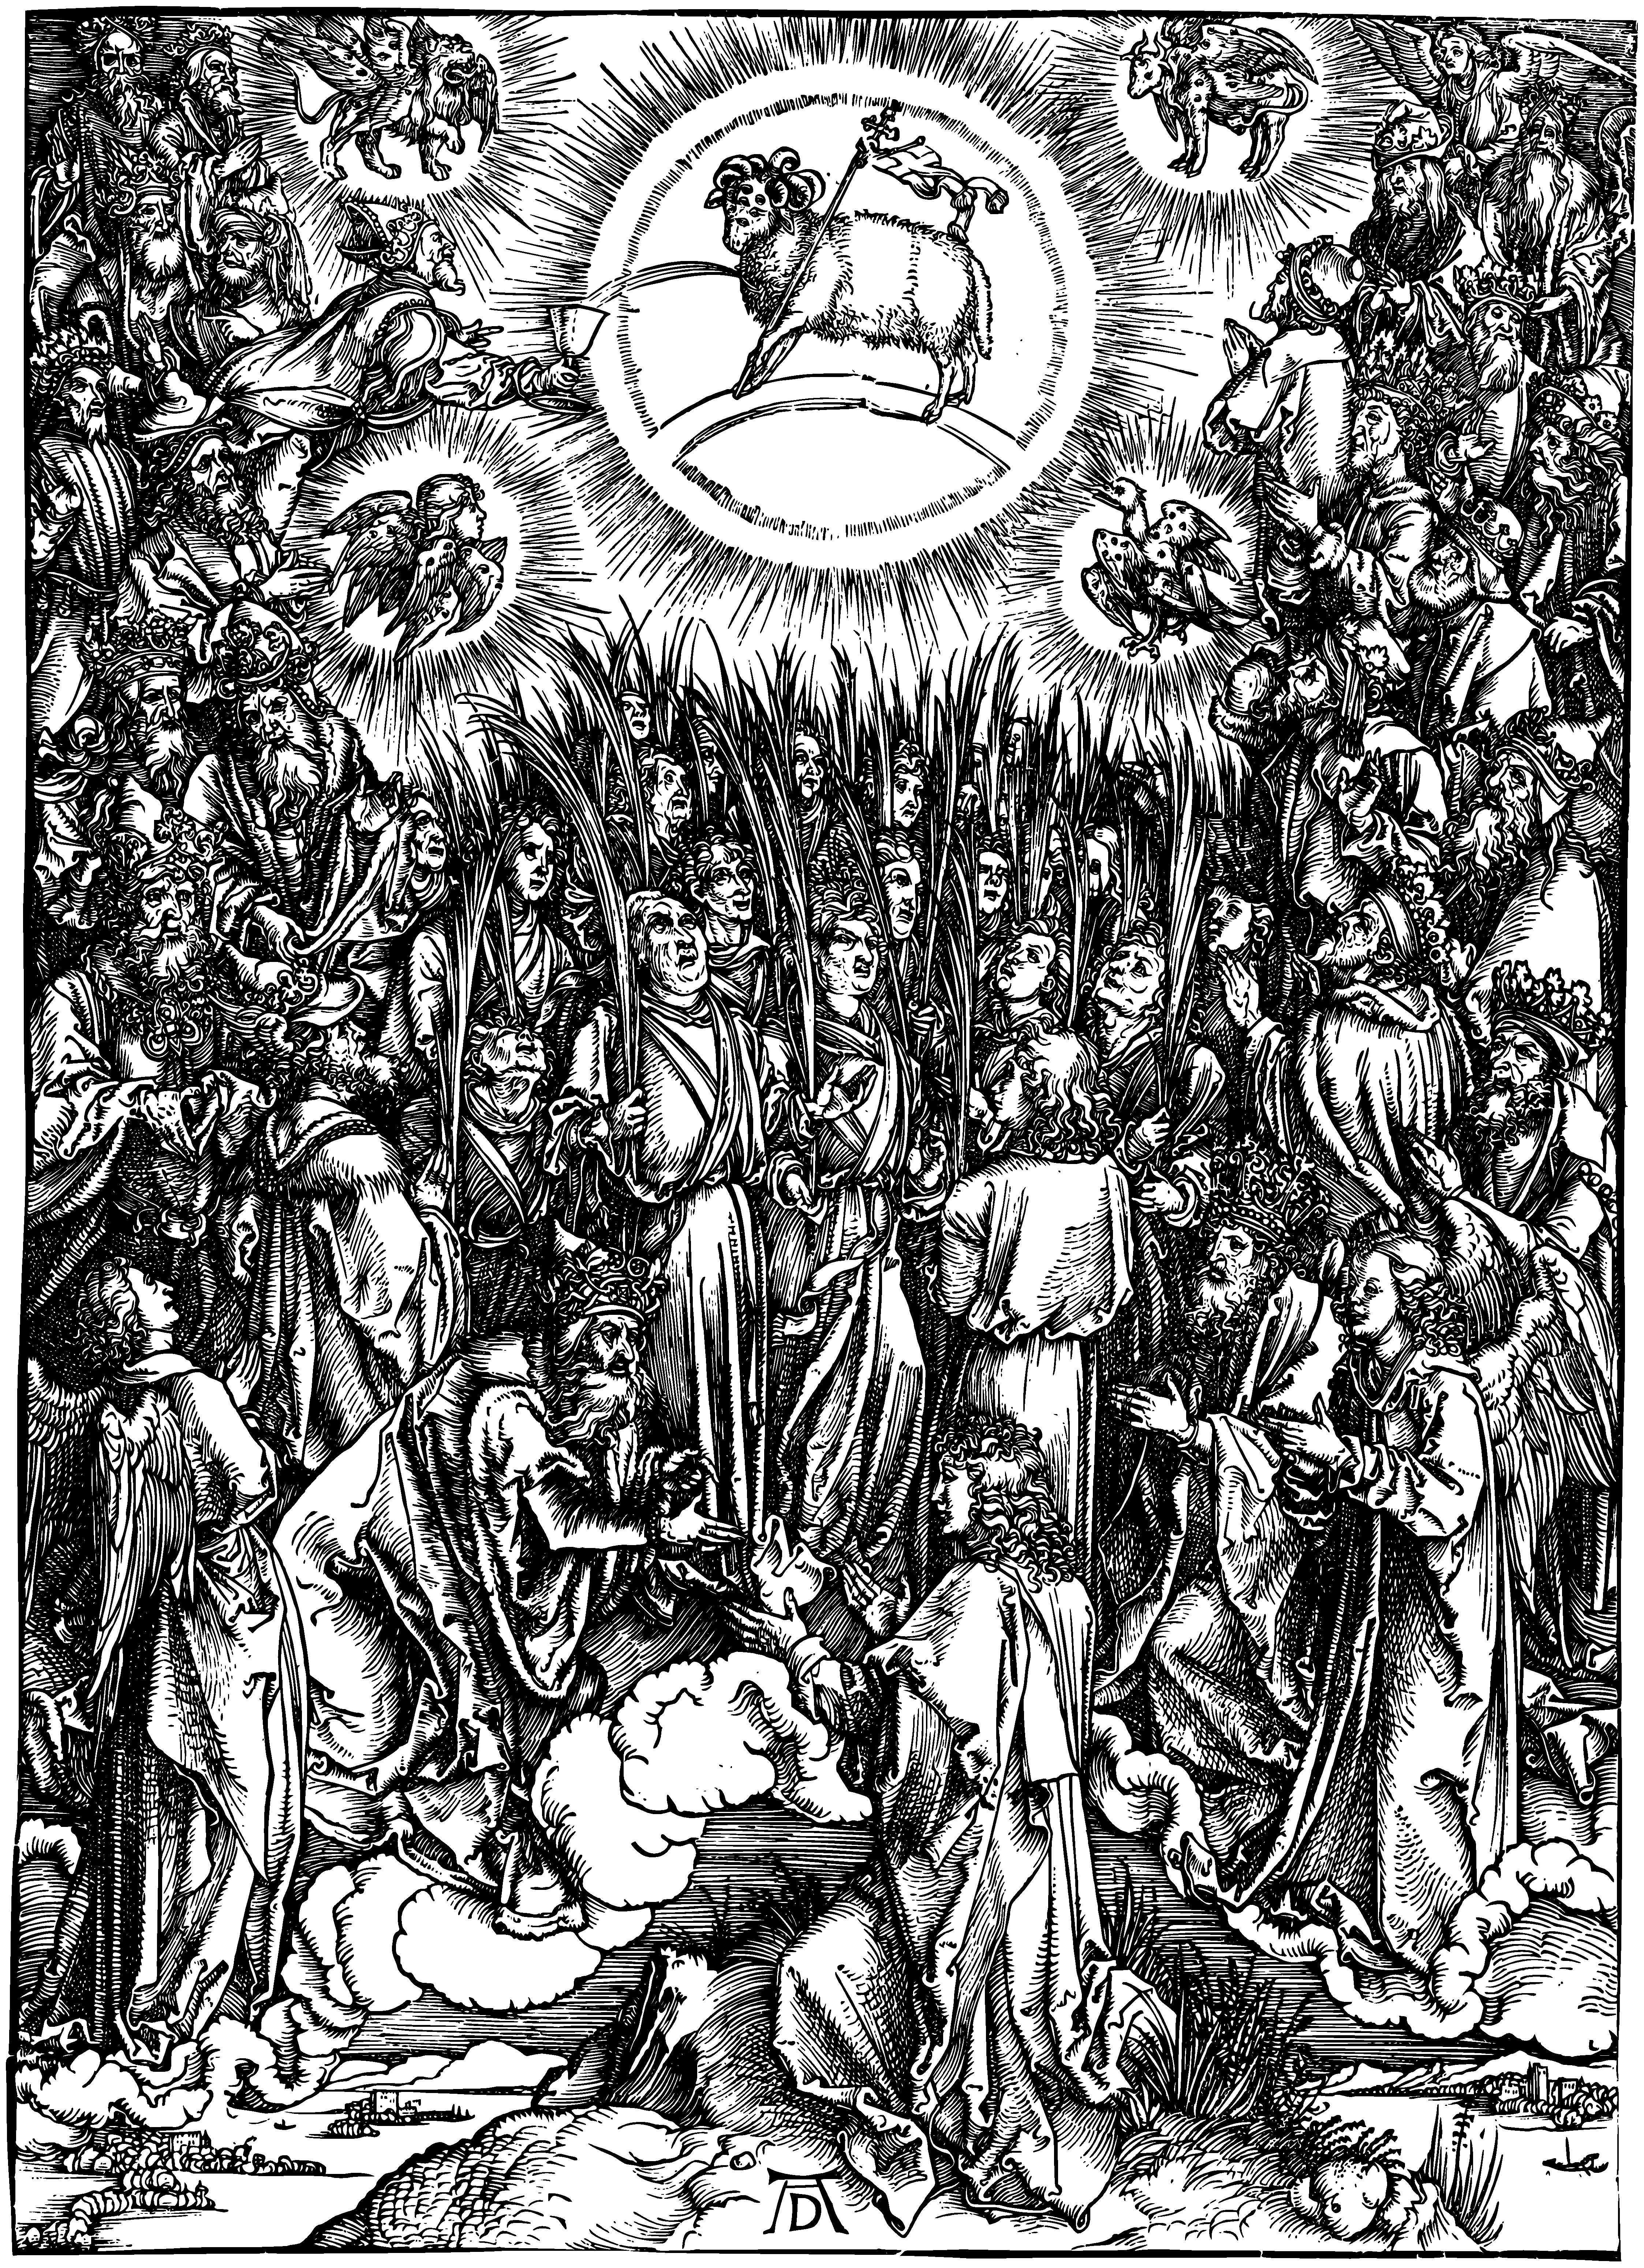
\includegraphics[width=98mm, height=140mm]{Apocalypse.eps}
    \caption{\textsc{\Huge{Devotional Hymns}}}
\end{figure}
   
\include{pages/Propers/DevotionalHymns.tex}
%Propers of Season and Saints
\cleardoublepage
\fancyhead[RE,LO]{}\fancyhead[RO,LE]{}
\fancyhead[C]{}\thispagestyle{empty}
\phantomsection
\addcontentsline{toc}{chapter}{Propers of the Church Year}

\begin{figure}[H]
    \centering
    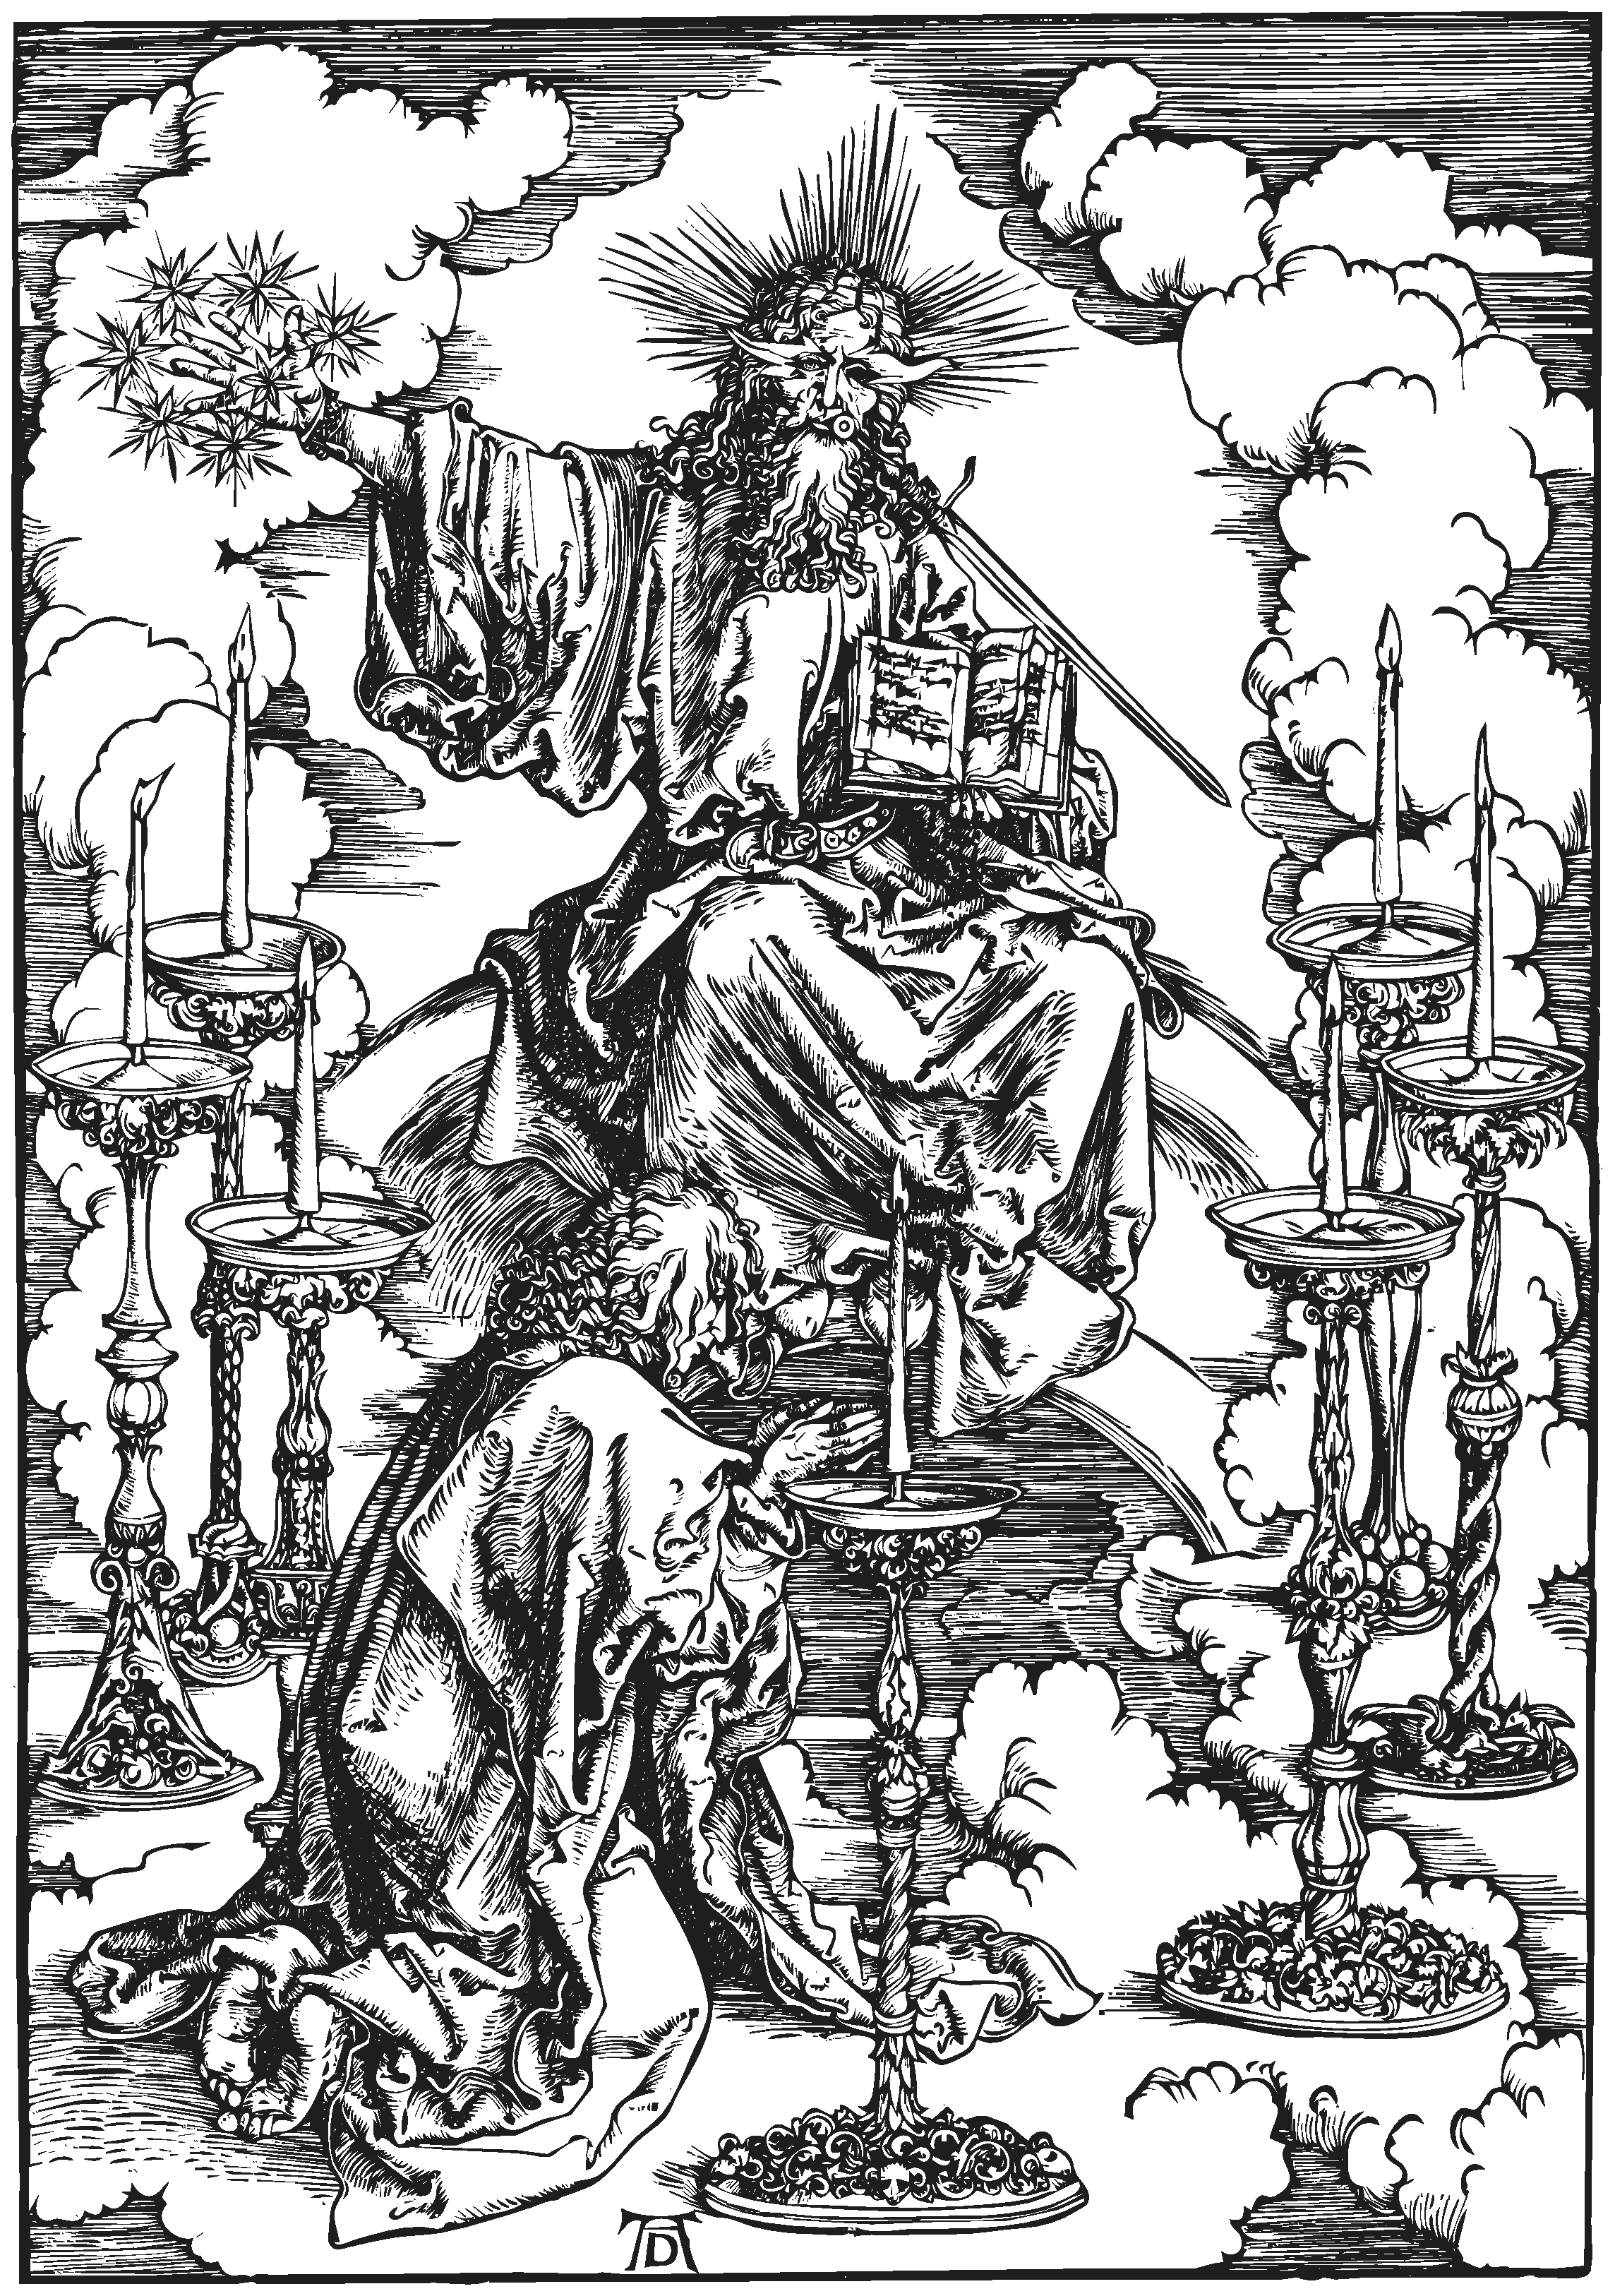
\includegraphics[width=98mm, height=140mm]{Vision.eps}
    \caption{\textsc{\Huge{Propers\\of the\\Church Year}}}
\end{figure}
\include{pages/Propers/HolyWeek.tex}
\include{pages/Propers/PropSeason.tex}
\include{pages/Propers/PropTime.tex}
%Common of Saints
\cleardoublepage
\include{pages/Propers/Commons.tex}
\include{pages/Propers/Common.tex}
%\subby{Seasonal Prayers}
\fancyhead[RO,LE]{\textit{Seasonal Prayers}}

   \subbysub{Of St. Mary in Advent}\label{SPMaryInAdvent}
   \begin{inhead}
   	Collect
   \end{inhead}
   \lett{O}{God,} who wast pleased that thy Word should take flesh of the womb of the blessed Virgin Mary at the message of an Angel: grant to thy humble servants; that we, who believe her to be truly the Mother of God, may be aided by her intercession in thy sight. Through the same.
  \begin{inhead}
  	Secret
  \end{inhead}
   \lett{W}{e} beseech thee, O Lord, stablish in our hearts the mysteries of thy true religion: that, as we believe thy Son, conceived of a Virgin, to be very God and very man; so by the power of his life-giving resurrection we may be found worthy to attain unto everlasting felicity. Through the same.
   \begin{inhead}
   	Postcommunion
   \end{inhead}
   \lett{W}{e} beseech thee, O Lord, pour thy grace into our hearts: that, as we have known the incarnation of thy Son Christ by the message of an Angel; so by his cross and passion we may be brought unto the glory of his resurrection. (Through the same.)


    \subbysub{Of St. Mary after Christmas}\label{SPMaryPostChristmas}
   \begin{inhead}
   	Collect
   \end{inhead}
    \lett{O}{God,} who by the virgin child-bearing of blessed Mary hast bestowed upon mankind the rewards of eternal salvation: grant, we beseech thee; that we may perceive her intercession for us, through whom we have been counted worthy to receive the author of life, Jesus Christ thy Son, our Lord. (Who liveth.)
  \begin{inhead}
  	Secret
  \end{inhead}
    \lett{T}{hrough} thy mercy, O Lord, and the intercession of blessed Mary ever Virgin, may this oblation avail for our prosperity and peace both now and for ever. (Through.)
   \begin{inhead}
   	Postcommunion
   \end{inhead}
    \lett{M}{ay} this communion, O Lord, cleanse us from guilt: and at the intercession of blessed Mary the Virgin Mother of God, make us partakers of thy heavenly healing. (Through the same.)
    
    
    \subbysub{Of St. Mary in Eastertide}\label{SPMaryInEaster}
   \begin{inhead}
   	Collect
   \end{inhead}
    \lett{G}{rant,} we beseech thee, O Lord God, that we thy servants may enjoy perpetual health of mind and of body: and, at the glorious intercession of blessed Mary ever Virgin, be delivered from present sadness, and rejoice in everlasting gladness. (Through.)
  \begin{inhead}
  	Secret
  \end{inhead}
    \lett{T}{hrough} thy mercy, O Lord, and the intercession of blessed Mary ever Virgin, may this oblation avail for our prosperity and peace, both now and ever. (Through.)
   \begin{inhead}
   	Postcommunion
   \end{inhead}
    \lett{G}{rant,} we beseech thee, O Lord: that we who have received these aids to our salvation may at all times and in all places be protected by the advocacy of blessed Mary ever Virgin; in whose honour we have made these offerings to thy Majesty. (Through.)\\

    \subbysub{Of Saints}\label{SPSaints}
   \begin{inhead}
   	Collect
   \end{inhead}
    \lett{D}{efend} us, O Lord, we beseech thee, from all dangers of mind and of body: and at the intercession of the blessed and glorious Mother of God, Mary ever Virgin, with blessed Joseph, thy blessed Apostles Peter and Paul, blessed \emph{N.}, and all the Saints, graciously grant us health and peace; that all adversities and errors being done away, thy Church may serve thee in freedom and quietness. (Through the same.)
  \begin{inhead}
  	Secret
  \end{inhead}
    \lett{G}{raciously} hear us, O God our Saviour: and by the power of this sacrament defend us from all enemies of mind and of body; granting us grace in this world, and glory in that which is to come. (Through.)
   \begin{inhead}
   	Postcommunion
   \end{inhead}
    \lett{W}{e} beseech thee, O Lord, that the gift now offered in this divine sacrament may cleanse and defend us: that at the intercession of blessed Mary the Virgin Mother of God, of blessed Joseph, of thy blessed Apostles Peter and Paul, of blessed \emph{N.} and of all the Saints; it may set us free from every perverse way, and deliver us from all adversities. (Through the same.)
    
   \subbysub{Against the Persecutors of the Church}\label{SPAgainst}
   \begin{inhead}
   	Collect
   \end{inhead}
   \lett{W}{e} beseech thee, O Lord, mercifully to hear the prayers of thy Church: that all adversities and errors being done away, she may serve thee in freedom and quietness. Through.
  \begin{inhead}
  	Secret
  \end{inhead}
   \lett{D}{efend} us, O Lord, who wait upon thy mysteries: that we, cleaving fast to things heavenly, may serve thee both in body and soul. Through.
   \begin{inhead}
   	Postcommunion
   \end{inhead}
   \lett{W}{e} beseech thee, O Lord our God: that we, whom thou makest to rejoice in the partaking of heavenly things, may by thee be defended against all earthly perils. Through.
   
   \subbysub{For the Chief Bishop}\label{SPChiefBishop}
   \begin{inhead}
   	Collect
   \end{inhead}
   \lett{O}{God,} the pastor and ruler of all the faithful, mercifully look upon thy servant \emph{N.}, whom thou hast been pleased to set as pastor over thy Church; grant him, we beseech thee, to be in word and conversation a wholesome example to the people committed to his charge; that he with them may attain unto everlasting life. Through.
  \begin{inhead}
  	Secret
  \end{inhead}
   \lett{L}{ook} favourably, we beseech thee, O Lord, upon the gifts which we offer: and guide with thy continual protection thy servant \textit{N.}, whom thou hast been pleased to set as pastor over thy Church. Through.
   \begin{inhead}
   	Postcommunion
   \end{inhead}
   \lett{W}{e} beseech thee, O Lord, that the divine sacrament which we have here received may be our protection: and together with the flock entrusted to his charge ever save and defend thy servant \textit{N.}; whom thou hast been pleased to set as pastor over thy Church. Through.
   
   \subbysub{Of the Holy Ghost}\label{SPHolyGhost}
   \begin{inhead}
   	Collect
   \end{inhead}
   \lett{G}{od,} who didst teach the hearts of thy faithful people, by the sending to them the light of thy Holy Spirit: grant us by the same Spirit to have a right judgment in all things; and evermore to rejoice in his holy comfort. (Through . . . in the unity of the same Holy Spirit.)
  \begin{inhead}
  	Secret
  \end{inhead}
   \lett{S}{anctify,} we beseech thee, O Lord, the gifts which we offer: and cleanse our hearts by the enlightening of the Holy Spirit. (Through . . . in the unity of the same Holy Spirit.)
   \begin{inhead}
   	Postcommunion
   \end{inhead}
   \lett{P}{our} thy Holy Spirit upon us, O Lord, and cleanse our hearts: that they may be made fruitful by the inward sprinkling of his dew. (Through . . . in the unity of the same Holy Spirit.)

    \subbysub{For the Living and Departed}\label{SPLivingDeparted}
   \begin{inhead}
   	Collect
   \end{inhead}
   \lett{A}{lmighty} and everlasting God, who hast dominion both of the living and of the dead, and hast mercy upon all who thou foreknowest will be thine in faith and works: we humbly beseech thee; that all those for whom we are minded to pour forth our prayers, whether in this present world they still be held in the flesh, or being delivered from the body have passed into that which is to come, may at the intercession of all thy Saints obtain of thy bountiful goodness the remission of all their sins. Through.
  \begin{inhead}
  	Secret
  \end{inhead}
   \lett{O}{God,} to whom alone is known the number of the elect, whom thou hast appointed unto heavenly felicity: grant, we beseech thee: that at the intercession of all thy Saints, the names of all those who have been commended to our prayers, and of all thy faithful people, may ever remain written in the book of those that are predestined to everlasting blessedness. Through.
   \begin{inhead}
   	Postcommunion
   \end{inhead}
   \lett{A}{lmighty} and merciful God, cleanse us, we pray thee, by the sacraments which we have received: and, at the intercession of all thy Saints, grant; that this thy sacrament may not bring upon us guilt to our punishment but pardon to our salvation: that it may cleanse away sins, that it may confirm the feeble, that it may defend us against every danger in this world: that it may obtain for thy faithful people both living and dead the remission of all their sins. Through.
%Hymn Index
\cleardoublepage
\include{pages/HymnIndex.tex}
%\cleardoublepage
\include{pages/Back.tex}
\end{document}
